\let\negmedspace\undefined{}
\let\negthickspace\undefined{}
\documentclass[journal,12pt,twocolumn]{IEEEtran}
 \usepackage{gensymb}
 \usepackage{polynom}
\usepackage{amssymb}
\usepackage[cmex10]{amsmath}
\usepackage{amsthm}
 \usepackage{stfloats}
\usepackage{bm} 
 \usepackage{longtable}
 \usepackage{enumitem}
 \usepackage{mathtools}
 \usepackage{tikz}
 \usepackage[breaklinks=true]{hyperref}
\usepackage{listings}
\usepackage{color}                                            
\usepackage{array}                                            
\usepackage{longtable}                                        
\usepackage{calc}                                             
    \usepackage{multirow}                                         
    \usepackage{hhline}                                           
    \usepackage{ifthen}                                           
    \usepackage{lscape}     
\DeclareMathOperator*{\Res}{Res}
\DeclareMathOperator*{\equals}{=}
\renewcommand\thesection{\arabic{section}}
\renewcommand\thesubsection{\thesection.\arabic{subsection}}
\renewcommand\thesubsubsection{\thesubsection.\arabic{subsubsection}}
\renewcommand\thesectiondis{\arabic{section}}
\renewcommand\thesubsectiondis{\thesectiondis.\arabic{subsection}}
\renewcommand\thesubsubsectiondis{\thesubsectiondis.\arabic{subsubsection}}
\hyphenation{op-tical net-works semi-conduc-tor}
\def\inputGnumericTable{}                                 %%
\lstset{ 
frame=single,
breaklines=true,
columns=fullflexible
}
\begin{document}
\newtheorem{theorem}{Theorem}[section]
\newtheorem{problem}{Problem}
\newtheorem{proposition}{Proposition}[section]
\newtheorem{lemma}{Lemma}[section]
\newtheorem{corollary}[theorem]{Corollary}
\newtheorem{example}{Example}[section]
\newtheorem{definition}[problem]{Definition}
\newcommand{\BEQA}{\begin{eqnarray}}
\newcommand{\EEQA}{\end{eqnarray}}
\newcommand{\define}{\stackrel{\triangle}{=}}
\newcommand*\circled[1]{\tikz[baseline= (char.base)]{
    \node[shape=circle,draw,inner sep=2pt] (char) {#1};}}
\bibliographystyle{IEEEtran}
\providecommand{\mbf}{\mathbf}
\providecommand{\pr}[1]{\ensuremath{\Pr\left(#1\right)}}
\providecommand{\qfunc}[1]{\ensuremath{Q\left(#1\right)}}
\providecommand{\sbrak}[1]{\ensuremath{{}\left[#1\right]}}
\providecommand{\lsbrak}[1]{\ensuremath{{}\left[#1\right.]}}
\providecommand{\rsbrak}[1]{\ensuremath{{}\left[#1\right.]}}
\providecommand{\brak}[1]{\ensuremath{\left(#1\right)}}
\providecommand{\lbrak}[1]{\ensuremath{\left(#1\right.)}
\providecommand{\rbrak}[1]{\ensuremath{\left[#1\right.]}}}
\providecommand{\cbrak}[1]{\ensuremath{\left\{#1\right\}}}
\providecommand{\lcbrak}[1]{\ensuremath{\left\{#1\right.}}
\providecommand{\rcbrak}[1]{\ensuremath{\left.#1\right\}}}
\theoremstyle{remark}
\newtheorem{rem}{Remark}
\newcommand{\sgn}{\mathop{\mathrm{sgn}}}
\providecommand{\abs}[1]{\left\vert#1\right\vert}
\providecommand{\res}[1]{\Res\displaylimits_{#1}} 
\providecommand{\norm}[1]{\left\lVert#1\right\rVert}
\providecommand{\mtx}[1]{\mathbf{#1}}
\providecommand{\mean}[1]{E\left[ #1 \right]}
\providecommand{\fourier}{\overset{\mathcal{F}}{ \rightleftharpoons}}
\providecommand{\system}{\overset{\mathcal{H}}{ \longleftrightarrow}}
\newcommand{\solution}{\noindent \textbf{Solution: }}
\newcommand{\cosec}{\,\text{cosec}\,}
\newcommand*{\permcomb}[4][0mu]{{{}^{#3}\mkern#1#2_{#4}}}
\newcommand*{\perm}[1][-3mu]{\permcomb[#1]{P}}
\newcommand*{\comb}[1][-1mu]{\permcomb[#1]{C}}
\renewcommand{\thetable}{\arabic{table}} 
\providecommand{\dec}[2]{\ensuremath{\overset{#1}{\underset{#2}{\gtrless}}}}
\newcommand{\myvec}[1]{\ensuremath{\begin{pmatrix}#1\end{pmatrix}}}
\newcommand{\mydet}[1]{\ensuremath{\begin{vmatrix}#1\end{vmatrix}}}
\numberwithin{equation}{section}
\numberwithin{figure}{section}
\numberwithin{table}{section} 
\makeatletter
\@addtoreset{figure}{problem}
\makeatother
\let\StandardTheFigure\thefigure{} 
\let\vec\mathbf{}
\def\putbox#1#2#3{\makebox[0in][l]{\makebox[#1][l]{}\raisebox{\baselineskip}[0in][0in]{\raisebox{#2}[0in][0in]{#3}}}}
     \def\rightbox#1{\makebox[0in][r]{#1}}
     \def\centbox#1{\makebox[0in]{#1}}
     \def\topbox#1{\raisebox{-\baselineskip}[0in][0in]{#1}}
     \def\midbox#1{\raisebox{-0.5\baselineskip}[0in][0in]{#1}}
\vspace{3cm}
\title{Random Numners}
\author{Gunjit Mittal (AI21BTECH11011)}
\maketitle
\tableofcontents
\section{Uniform Random Numbers}
\begin{enumerate}[label=\thesection.\arabic*
,ref=\thesection.\theenumi]
    \item
    \begin{figure}[h]
        \centering
        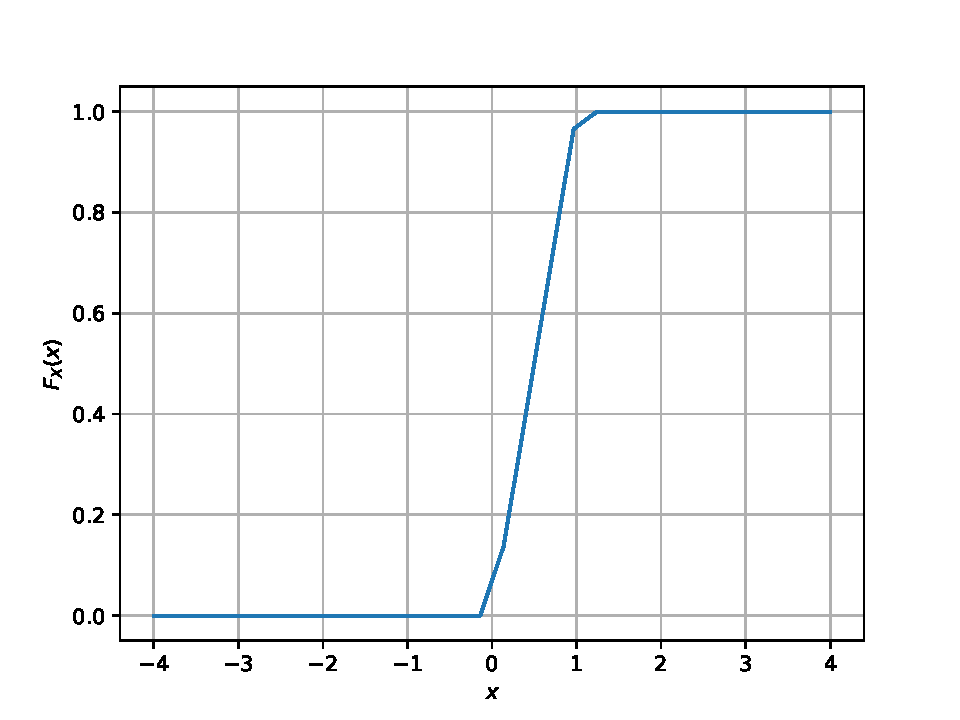
\includegraphics[width=\columnwidth]{../figs/uni_cdf}
        \caption{The CDF of $U$}\label{fig:uni_cdf}
        \end{figure}
    \item
    \item \solution{}Since U is  a uniform distribution
    \begin{align}
        F_U(x) = x
    \end{align}
    \item
    \item Verify your result theoretically given that
    \end{enumerate}
    %
    \begin{equation}
    E\sbrak{U^k} = \int_{-\infty}^{\infty}x^k dF_{U}(x)
    \end{equation}
    \begin{align}
        &E\sbrak{U} = \int_{-\infty}^{\infty}x dF_U(x)\\
        &~~~~~= \int_{0}^{1}x dx\\
        &~~~~~= \sbrak{\frac{x^2}{2}}^1_0\\
        &~~~~~= \frac{1}{2}
    \end{align}
    \begin{align}
        &E\sbrak{U-E\sbrak{U}}^2 = E\sbrak{U^2} - E\sbrak{U}^2\\
        &E\sbrak{U^2} = \int_{-\infty}^{\infty}x^2 dF_U(x)\\
        &~~~~~= \int_{0}^{1}x^2 dx\\
        &~~~~~= \sbrak{\frac{x^3}{3}}^1_0\\
        &~~~~~= \frac{1}{3}\\
        &E\sbrak{U-E\sbrak{U}}^2 =  \frac{1}{3} - \brak{\frac{1}{2}}^2\\
        &~~~~~~ = \frac{1}{3} - \frac{1}{4}  =\frac{1}{12}
    \end{align}
    \section{Central Limit Theorem}
    %
    \begin{enumerate}[label=\thesection.\arabic*
,ref=\thesection.\theenumi]
    %
    \item
    \item 
    \begin{figure}[h]
        \centering
        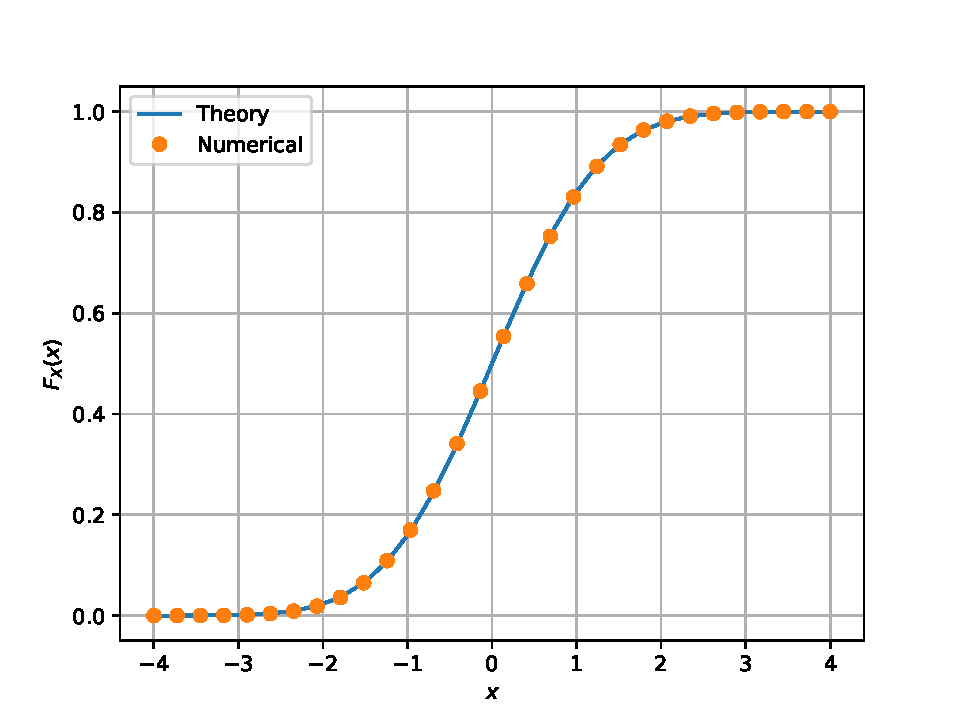
\includegraphics[width=\columnwidth]{../figs/gauss_cdf}
        \caption{The CDF of $X$}\label{fig:gauss_cdf}
        \end{figure}
    \item\solution{}
    \begin{itemize}
        \item PDF is symmetric about x=0\\ 
        \item Graph is bell shaped\\
        \item Mean of graph is situated at the apex point of the bell.
    \end{itemize}
    \begin{figure}[h]
    \centering
    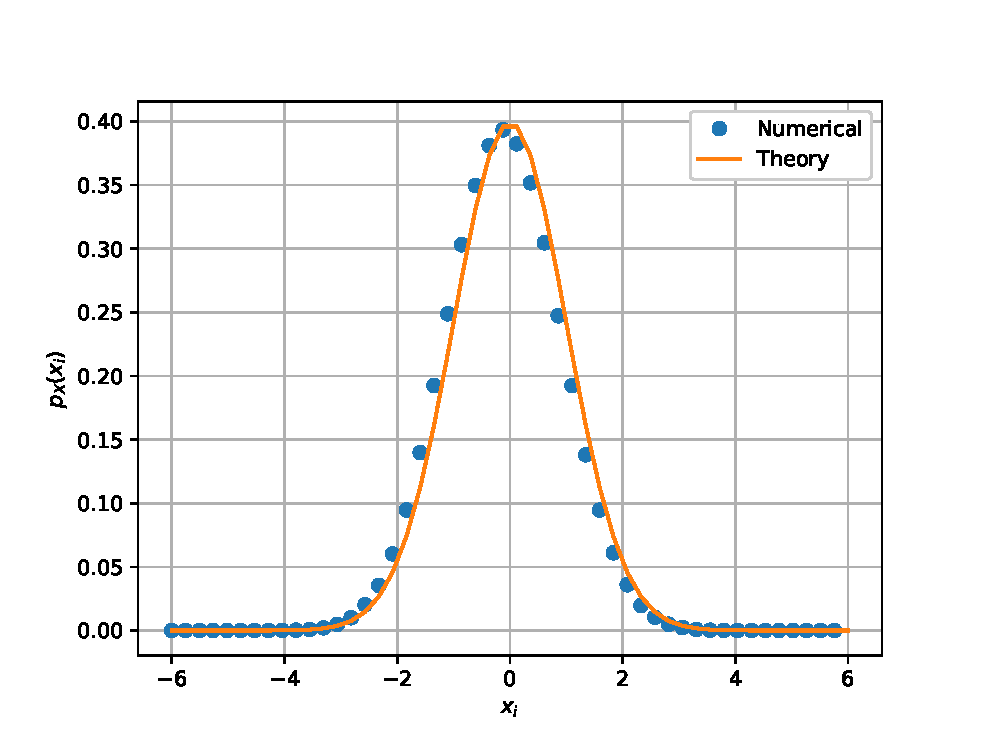
\includegraphics[width=\columnwidth]{../figs/gauss_pdf}
    \caption{The PDF of $X$}\label{fig:gauss_pdf}
    \end{figure}
    \item
    \item \begin{align}
        &F_X(x) = \int_{-\infty}^{x} \frac{1}{\sqrt[]{2\pi}}e^{-\frac{x^2}{2}}\\
        &~~~~~~~= \frac{1}{2} erf(\frac{x}{\sqrt[]{2}})\\
        &E[X] = \frac{1}{\sqrt[]{2\pi}}\int_{-\infty}^{\infty}xe^{-\frac{x^2}{2}}dx\\
        &\text{Taking  }\frac{x^2}{2} = t \implies x dx = dt\\
        &E[X] = \frac{1}{\sqrt[]{2\pi}}\int_{\infty}^{\infty}e^{-t}dt = 0\\
        &E[X^2]=\int_{-\infty}^{\infty} \frac{1}{\sqrt{2\pi}} x^2e^{-\frac{x^2}{2}} dx\\
        &~~~~~~=\frac{1}{\sqrt{2\pi}}\int_{-\infty}^{\infty}  x(xe^{-\frac{x^2}{2}}) dx\\
        &~~~~~~~= \frac{1}{\sqrt{2\pi}} \sbrak{-xe^{-\frac{-x^2}{2}}+\int_{-\infty}^{\infty} e^{-\frac{x^2}{2}} dx}^{\infty}_{-\infty}\\
        &~~~~~~~= 1\\
        &\text{Variance} = E[X^2] - {E[X]}^2 = 1 - 0 = 1
    \end{align}
    %
    \end{enumerate}
    \section{From Uniform to Other}
    \begin{enumerate}[label=\thesection.\arabic*,ref=\thesection.\theenumi]
    %
    \item
    \begin{figure}
        \centering
        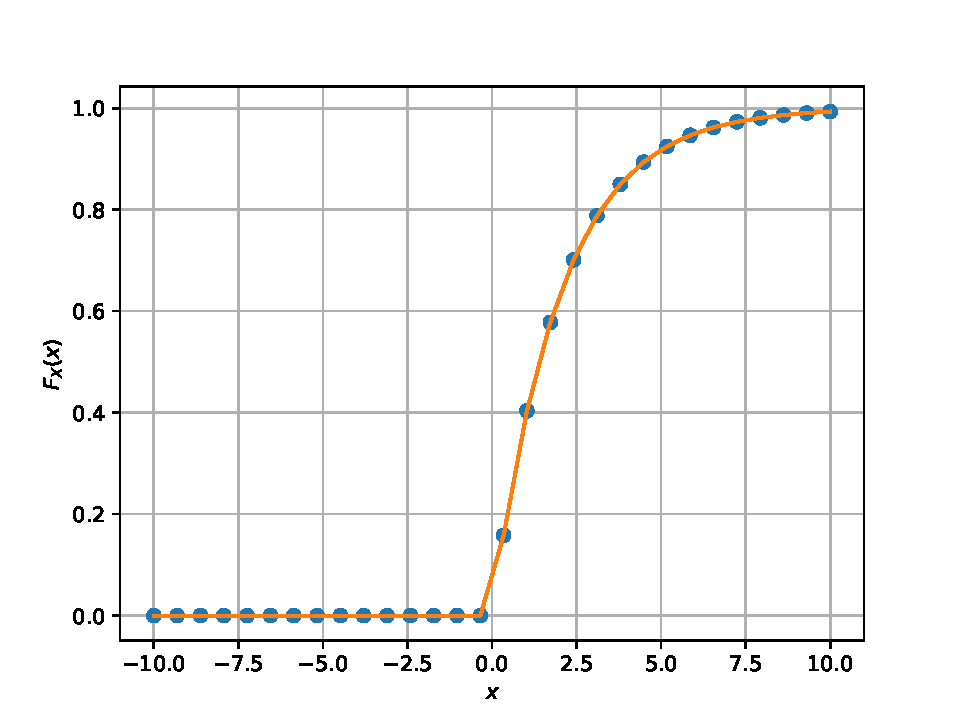
\includegraphics[width=\columnwidth]{../figs/V_cdf}
        \caption{The CDF of $V$}\label{fig:V_cdf}
        \end{figure}
    \item \begin{align}
        &F_{V}(x)=P(V \leq x)\\
        &~~~~~~~~=P(-2 \ln (1-U) \leq x)\\
        &~~~~~~~~=P(U \leq 1-e^{\frac{-x}{2}})\\
        &P(U<x)=\int_{0}^{x} dx=x\\
        &\therefore P(U \leq 1-e^{\frac{-x}{2}})=1-e^{\frac{-x}{2}} \\ 
        &\implies F_{V}(x) = 1-e^{\frac{-x}{2}}
        \end{align}
    %
    %\item
    %Generate the Rayleigh distribution from Uniform. Verify your result through graphical plots.
    \end{enumerate}
    
\end{document}  